\documentclass[runningheads]{llncs}

\usepackage{graphicx}
\usepackage{hyperref}
\usepackage{multicol}

%%%%%%%%%%%%%%%%%%%%%%%%%%%%%%%%%%%%%%%%%%%%%%%%%%%%%%

\begin{document}
\title{Inequality of opportunity in the research career: a quantitative analysis.}
\author{Alberto Morales Galán
\and
Oriol Colomé Font}
%%%%%%%%%%%%%%%%%%%%%%%%%%%%%%%%%%%%%%%%%%%%%%%%%%%%%%
\institute{Universitat Pompeu Fabra, Barcelona \and
\email{\{alberto.morales01, oriol.colome01\}@estudiant.upf.edu}\\
\url{http://www.upf.edu}}
%%%%%%%%%%%%%%%%%%%%%%%%%%%%%%%%%%%%%%%%%%%%%%%%%%%%%%
\maketitle              % typeset the header of the contribution
%%%%%%%%%%%%%%%%%%%%%%%%%%%%%%%%%%%%%%%%%%%%%%%%%%%%%%
\begin{abstract}
Meta-research analysis. Where is the spotlight shining on when it comes to inequality of opportunity in the research career? Where does the academia invest their resources when studying the phenomenon? 
We strive to address one of the most important ethical issues in academia today: equality of opportunity. By identifying known factors of discrimination we looked at where most of the research efforts are channelled into when investigating the issue of inequality of opportunity in the research career.

\keywords{Discrimination \and Inequality \and Equality \and Discrimination in science  \and Inequality in science \and Research career}
\end{abstract}
%%%%%%%%%%%%%%%%%%%%%%%%%%%%%%%%%%%%%%%%%%%%%%%%%%%%%%
%%%%%%%%%%%%%%%%%%%%%%%%%%%%%%%%%%%%%%%%%%%%%%%%%%%%%%
%%%%%%%%%%%%%%%%%%%%%%%%%%%%%%%%%%%%%%%%%%%%%%%%%%%%%%
\section{Introduction}
Social protest movements such as \href{https://hipatiapress.com/hpjournals/index.php/hse/article/view/10545/3659}{\#MeToo} or \href{https://doi.org/10.1016/j.jnma.2021.12.009}{\#BlackLivesMatter} have highlighted the need for greater diversity, equity, and inclusion at scientific institutions worldwide. In this article, we decided to conduct a meta-research analysis to find where the spotlight is shining regarding inequality of opportunity in the research career in order to spot the academia's coverage of the phenomenon.

\begin{definition}
\href{https://languages.oup.com/}{Discrimination} is the unjust or prejudicial treatment of different categories of people.
\end{definition}
%%%%%%%%%%%%%%%%%%%%%%%%%%%%%%%%%%%%%%%%%%%%%%%%%%%%%%
\subsection{Research question(s)}
Are there situations of discrimination when accessing a research career? If so, what are the possible causes of that discrimination? When studying this phenomenon, what has been the general tendency for the past five years?
%%%%%%%%%%%%%%%%%%%%%%%%%%%%%%%%%%%%%%%%%%%%%%%%%%%%%%
\section{Methodology}
We used the \href{https://www.scopus.com/}{SCOPUS} search tool to do all tasks above, which contains an extensive database of multidisciplinary scientific publications.
\subsection{SCOPUS}
SCOPUS uniquely combines a comprehensive, expertly curated abstract and citation database with enriched data and linked scholarly literature across various disciplines. It quickly finds relevant and authoritative research, identifies experts, and provides access to reliable data, metrics, and analytical tools.
%%%%%%%%%%%%%%%%%%%%%%%%%%%%%%%%%%%%%%%%%%%%%%%%%%%%%%
\subsection{Research procedure}
We based the procedure of our analysis on selecting a set of articles that met the condition of dealing with discrimination in academia for \textbf{any} cause and then analyzing how many articles were related to which types of discrimination. 

Defining a data-set \textbf{beforehand} instead of searching for publications on each type of discrimination, had an apparent aim: avoiding the introduction of bias in our analysis.

\subsection{Set of publications to be analyzed} 
We defined our inclusion criteria as those contained in the \textit{title/abstract}: \textbf{inequality}, \textbf{discrimination}, or \textbf{equality}. We also included words and concepts such as \textbf{academic career} and \textbf{research career}. From the initial set of publications, we analyzed how many of them dealt with discrimination based on gender, race, and sexual orientation. This analysis was also performed by searching for keywords in the title or abstract of the publications. 

%\subsubsection{}
\subsubsection{SCOPUS QUERY}
\textit{( TITLE-ABS-KEY (inequality) OR TITLE-ABS-KEY-AUTH (equality) OR TITLE-ABS-KEY (discrimination)) AND (TITLE-ABS-KEY ("academic career") OR TITLE-ABS-KEY-AUTH ("research career") OR TITLE-ABS-KEY-AUTH ("researcher career")) and not (TITLE-ABS-KEY (women) or TITLE-ABS-KEY (machism) or TITLE-ABS-KEY (race) or TITLE-ABS-KEY (racial) or TITLE-ABS-KEY (ethnic) or TITLE-ABS-KEY (lgtbq) or TITLE-ABS-KEY (lgbtq) or TITLE-ABS-KEY (homosexual) or TITLE-ABS-KEY (homosexuality) or TITLE-ABS-KEY (gay) or TITLE-ABS-KEY (lesbian)) AND ( EXCLUDE ( DOCTYPE,"ch" ) OR EXCLUDE ( DOCTYPE,"bk"))}

\subsubsection{}
After analyzing the most common types of discrimination, we discarded these papers. Then, we analyzed the remaining ones in search of other types of discrimination. This search was performed by selecting a random sample of papers and analyzing their subject matter. We carried the procedure out iteratively until no new causes of discrimination could be determined, at which point we ended the search. 

%%%%%%%%%%%%%%%%%%%%%%%%%%%%%%%%%%%%%%%%%%%%%%%%%%%%%%
\subsection{Academia tendency for the past five years: text analysis}
We scrapped the PDF selection using \href{https://www.python.org/}{Python} and then processed the data with common data handling libraries and Natural Language Processing tools such as \href{https://pandas.pydata.org/}{Pandas} and \href{https://www.nltk.org/}{NLTK}. 

To achieve a clean text to work with, we removed all special characters and punctuation; we also erased the English stop-words. Stop-words are available in abundance in any human language. By removing these words, we remove the low-level information from our text in order to give more focus to the high-level information. The complete Google Colab Notebook can be found  \href{https://colab.research.google.com/drive/1IjIltXAYM-fAM2dUuPyqpsezf4HZf19G?usp=sharing}{here.}
%%%%%%%%%%%%%%%%%%%%%%%%%%%%%%%%%%%%%%%%%%%%%%%%%%%%%%
\section{Results}
\subsection{SCOPUS Query Search}
Two hundred eighty-four articles met the criteria for inclusion in the analysis. Of these 284, 220 articles dealt with \textbf{gender discrimination}, 24 with \textbf{racial discrimination}, and only 2 with \textbf{sexual orientation discrimination}. 

Subsequent analysis of the remaining 38 articles allowed us to find the following causes of discrimination: socioeconomic conditions, age, and disability. We found 14 publications on \textbf{social class conditions}, six on \textbf{ageism}, and five articles on \textbf{disability}. The remaining 13 articles were analyzed, but we did not find new types of discrimination.
%%%%%%%%%%%%%%%%%%%%%%%%%%%%%%%%%%%%%%%%%%%%%%%%%%%%%%
\begin{table}
\caption{Number of articles found per discrimination cause based on the searching criteria.}\label{tab1}
\centering
\begin{tabular}{|l|l|}
\hline
Discrimination cause & Number of articles\\
\hline
Gender (sexism) & 220 \\
Race (racism) & 24 \\
Socioeconomic status (SES) & 14 \\
Other & 13 \\
Age (ageism) & 6 \\
Disability (ableism) & 5 \\
Sexual orientation (\href{https://www.collinsdictionary.com/dictionary/english/sexualism}{sexualism}) & 5 \\ 
\hline
\end{tabular}
\end{table}
%%%%%%%%%%%%%%%%%%%%%%%%%%%%%%%%%%%%%%%%%%%%%%%%%%%%%%
\subsection{Tendency study}
Regarding the tendency study, only 66,55\% of the articles found in SCOPUS were open access. Therefore, we only applied the quantitative analysis of the word occurrences on this ~67\% accessible sample.
%%%%%%%%%%%%%%%%%%%%%%%%%%%%%%%%%%%%%%%%%%%%%%%%%%%%%%
\begin{table}
\caption{Number of Open Access PDF per year within selection}\label{tab2}
\centering
\begin{tabular}{|l|l|}
\hline
Year of publication & Open Access PDF\\
\hline
2019 & 19 \\
2020 & 47 \\
2021 & 64 \\
2022 & 59 \\
\hline
\end{tabular}
\end{table}

The results are displayed in \textbf{Table 3}\textit{} \ref{tab3} as well as plotted in \textbf{Figure 1}\textit{} \ref{chart}
%%%%%%%%%%%%%%%%%%%%%%%%%%%%%%%%%%%%%%%%%%%%%%%%%%%%%%
\begin{table}
\caption{Number of word occurrences per year of study within selection}\label{tab3}
\centering
\begin{tabular}{|l|l|l|l|l|}
\hline
Word &  2019 & 2020 & 2021 & 2022\\
\hline
age & 63 & 189 & 245 & 227 \\
ageism & 0 & 0 & 1 & 1 \\
disability & 1 & 5 & 63 & 157 \\
discrimination & 39 & 168 & 290 & 244 \\
equality & 35 & 42 & 196 & 121 \\ 
ethnic & 12 & 37 & 50 & 106 \\
gay & 2 & 23 & 4 & 5 \\
gender &122 &274 &741 &613 \\
heterosexual &0 &4 &6 &4 \\
homosexual &2 &0 &0 &0 \\
inequality &101 &79 &204 &184 \\
lesbian &0 &12 &5 &6 \\
lgtbq &0 &1 &0 &0 \\
machismo &0 &0 &1 &0 \\old &18 &46 &53 &73 \\
race &19 &99 &99 &102 \\
racial &12 &24 &43 &75 \\
racism &0 &12 &25 &199 \\
racist &0 &2 &9 &26 \\
socioeconomic &22 &26 &24 &34 \\
woman &4 &10 &41 &68 \\
young &22 &123 &195 &204 \\
\hline
\end{tabular}
\end{table}
%%%%%%%%%%%%%%%%%%%%%%%%%%%%%%%%%%%%%%%%%%%%%%%%%%%%%%
\begin{figure}
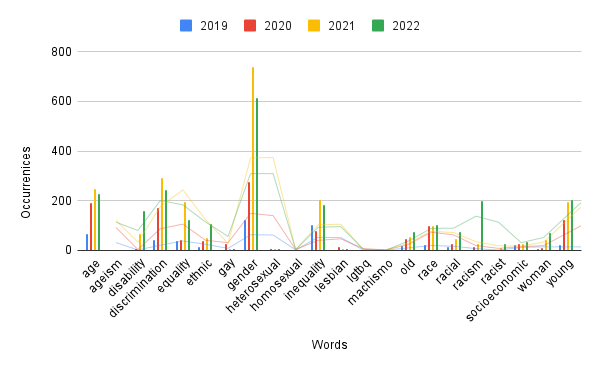
\includegraphics[width=\textwidth]{chart.png}
\centering
\caption{Number of word occurrences per year of study.} \label{chart}
\end{figure}
%%%%%%%%%%%%%%%%%%%%%%%%%%%%%%%%%%%%%%%%%%%%%%%%%%%%%%

\section{Discussion}
According to the results obtained from the analysis, we can conclude that the main object of the study is gender discrimination, representing more than 75\% of all the analyzed articles. It is also clear that the number of articles studying this type of phenomenon has a growing tendency, not to say its number increases yearly. It shows a concern that researchers themselves try to detect and describe. The slight drop in 2022 does not appear significant at first glance\ref{tab2}.

While it is true that the distribution of articles has increased across all types of discrimination, in the case of racial discrimination, it is particularly significant. This particularly sharp increase seems to indicate that there has been a recent increase in interest in racial discrimination in academia, possibly due to the impact of movements such as \href{https://doi.org/10.1016/j.jnma.2021.12.009}{\#BlackLivesMatter} that developed shortly before this increase.

According to the scientific literature we based the research on, there is also an iterative element: the crucial role played by the institutions when it comes to remedying this type of situation. From our point of view, it is noteworthy to highlight the possible relationship between these last two conclusions: the academic environment is interested in addressing such a funding problem.

This perspective is a silver lining. The future outlook on discrimination in academia may be bright. According to the results of \href{https://doi.org/10.1111/gwao.12549}{recent studies}, these changes in more egalitarian academia may have already begun to have an impact since these researchers detected a decrease in the gender gap among post-doc students, which was not reflected among faculty. In other words, these measures that can be taken at the institutional level have already begun to affect the younger generations. They will gradually permeate the rest of the university and research institutes.

\begin{multicols}{2}
[]
\section{References}
\scriptsize
Charlotte Silander, Ulrika Haake, Leif Lindberg, \& Ulla Riis (2022). Nordic research on gender equality in academic careers: a literature review. European Journal of Higher Education, 12, 72-97.

Joana Vicente, Kevin J. McKee, Lennart Magnusson, Pauline Johansson, Björn Ekman, \& Elizabeth Hanson (2022). Informal care provision among male and female working carers: Findings from a Swedish national survey. PLoS ONE, 17.

Anne Marie Weber-Main, Jeffrey Engler, Richard McGee, Marlene J. Egger, Harlan P. Jones, Christine V. Wood, Kristin Boman, Jiqiang Wu, Andrew K. Langi, \& Kolawole S. Okuyemi (2022). Variations of a group coaching intervention to support early-career biomedical researchers in Grant proposal development: a pragmatic, four-arm, group-randomized trial. BMC Medical Education, 22.

Ascanio Tridente, Jack Parry-Jones, Shashi Chandrashekaraiah, \& Daniele Bryden (2022). Differential attainment and recruitment to Intensive Care Medicine Training in the UK, 2018–2020. BMC Medical Education, 22.

Sergio Villanueva Baselga, Oriol Marimon Garrido, \& Helena González Burón (2022). Drama-Based Activities for STEM Education: Encouraging Scientific Aspirations and Debunking Stereotypes in Secondary School Students in Spain and the UK. Research in Science Education, 52, 173-190.

Valentina S. Consiglio, \& Denisa M. Sologon (2022). The Myth of Equal Opportunity in Germany? Wage Inequality and the Role of (Non-)academic Family Background for Differences in Capital Endowments and Returns on the Labour Market. Social Indicators Research, 159, 455-493.

Kate Bancroft, \& Scott Greenspan (2022). Facilitators and barriers of inclusion: a critical incident technique analysis of one non-binary Physical Education teacher’s workplace experiences. Sport, Education and Society.

Ana María Yáñez-Serrano, Maricar Aguilos, Cybelli Barbosa, Tomás Rafael Bolaño-Ortiz, Samara Carbone, Stephanie Díaz-López, Sebastián Diez, Pamela Dominutti, Vanessa Engelhardt, Eliane Gomes Alves, Jenniffer Pedraza, Jorge Saturno, \& Zitely A. Tzompa-Sosa (2022). The Latin America Early Career Earth System Scientist Network (LAECESS): addressing present and future challenges of the upcoming generations of scientists in the region. npj Climate and Atmospheric Science, 5.

Sonia Verdugo-Castro, Mª ªC Sánchez-Gómez, \& Alicia García-Holgado (2022). University students’ views regarding gender in STEM studies: Design and validation of an instrument. Education and Information Technologies.

Jouni Helin, Juho Jokinen, Kristian Koerselman, Terhi Nokkala, \& Eija Räikkönen (2022). It runs in the family?: Using sibling similarities to uncover the hidden influence of family background in doctoral education and academic careers. Higher Education.

Chiara Corvino, Amalia De Leo, Miriam Parise, \& Giulia Buscicchio (2022). Organizational Well-Being of Italian Doctoral Students: Is Academia Sustainable When It Comes to Gender Equality?. Sustainability (Switzerland), 14.

Susan Smith, \& David Walker (2022). Scholarship and teaching-focused roles: An exploratory study of academics’ experiences and perceptions of support. Innovations in Education and Teaching International.

Cecile B. Menard, \& Sara Shinton (2022). The career paths of researchers in long-term employment on short-term contracts: Case study from a UK university. PLoS ONE, 17.

Hans Jonker, Florian Vanlee, \& Walter Ysebaert (2022). Societal impact of university research in the written press: media attention in the context of SIUR and the open science agenda among social scientists in Flanders, Belgium. Scientometrics.

Johanne Mathieu, Salomon Fotsing, Kikelomo Akinbobola, Lolade Shipeolu, Kien Crosse, Kimberley Thomas, Manon Denis-LeBlanc, Abdoulaye Gueye, \& Gaelle Bekolo (2022). The quest for greater equity: a national cross-sectional study of the experiences of Black Canadian medical students. CMAJ open, 10, E937-E944.

Annamaria Di Fabio, \& Andrea Svicher (2022). Precariousness in the time of COVID-19: A turning point for reforming and reorganizing career counselling for vulnerable workers. Cypriot Journal of Educational Sciences, 17, 1477-1494.

Myia S. Williams, Alyson K. Myers, Kayla D. Finuf, Vidhi H. Patel, Lyndonna M. Marrast, Renee Pekmezaris, \& Johanna Martinez (2022). Black Physicians’ Experiences with Anti-Black Racism in Healthcare Systems Explored Through An Attraction-Selection-Attrition Lens. Journal of Business and Psychology.

Agnieszka Fudali-Czyż, Piotr Janusz Mamcarz, Klaudia Martynowska, Ewa Domagała-Zyśk, \& Andrew Rothwell (2022). Sex differences in self-perceived employability and self-motivated strategies for learning in Polish first-year students. PLoS ONE, 17.

Sebastian C.K. Shaw, Lucy Jane Davis, \& Mary Doherty (2022). Considering autistic patients in the era of telemedicine: the need for an adaptable, equitable, and compassionate approach. BJGP Open, 6, 1-4.

Justin B. Dimick, Jeffrey B. Matthews, \& Douglas E. Wood (2022). Department of Surgery Leadership Towards Diversity, Equity, and Inclusion. Current Trauma Reports.

Jasmin Graham, Gina Hodsdon, Aly Busse, \& Michael P. Crosby (2022). BIPOC voices in ocean sciences: A qualitative exploration of factors impacting career retention. Journal of Geoscience Education.

Hazel McCafferty (2022). An unjust balance: a systematic review of the employability perceptions of UK undergraduates from disadvantaged socio-economic backgrounds. Research in Post-Compulsory Education, 27, 570-593.

Claudia Schuchart, \& Benjamin Schimke (2022). Age and Social Background as Predictors of Dropout in Second Chance Education in Germany. Adult Education Quarterly, 72, 308-328.

Erika Collie, Raelia Lew, \& Michelle Peate (2022). Merging motherhood and medicine: A qualitative study exploring barriers and enablers to motherhood among female doctors in Australia. Women's Health, 18.

Cecilia Tallatta, \& Lucía Romero Massobrio (2022). Editors' notes: Addressing linguistic inequality in Latin America. Sociolinguistic and ethnographic approaches to study the uses of indigenous languages in education. Bellaterra Journal of Teaching and Learning Language and Literature, 15.

Katherine Sang, Thomas Calvard, \& Jennifer Remnant (2022). Disability and Academic Careers: Using the Social Relational Model to Reveal the Role of Human Resource Management Practices in Creating Disability. Work, Employment and Society, 36, 722-740.

Melissa Haeffner, Dana Hellman, Alida Cantor, Idowu Ajibade, Vinka Oyanedel-Craver, Maura Kelly, Laura Schifman, \& Lisa Weasel (2021). Representation justice as a research agenda for socio-hydrology and water governance. Hydrological Sciences Journal, 66, 1611-1624.

Lee Ann Sutherland, Rob J.F. Burton, Anda Adamsone-Fiskovica, Claire Hardy, Boelie Elzen, Lies Debruyne, \& Sharon Flanigan (2021). Inclusivity of on-farm demonstration: gender, age, and geographic location. Journal of Agricultural Education and Extension, 27, 591-613.

Ana Belén Herranz Sánchez, Carmen Rísquez Cuenca, Carmen Rueda Galán, \& Francisca Hornos Mata (2021). Iberian Heritage Routes and Itineraries. A Reflection from Feminist Archaeology. Complutum, 32, 601-621.

Philipp Aufenvenne, Christian Haase, Franziska Meixner, \& Malte Steinbrink (2021). Gender Relations at a Geographical Congress. Participation and Communication at the German Geographical Congress in Kiel (2019). Mitteilungen der Osterreichischen Geographischen Gesellschaft, 163, 29-59.

Katherine Weisshaar (2021). Employment Lapses and Subsequent Hiring Disadvantages: An Experimental Approach Examining Types of Discrimination and Mechanisms. Socius, 7.

Aisha Yaghmour, Alaa Alesa, Esraa Anbarserry, Merihan Abdullah Binmerdah, Ahlam Alharbi, Abdulrahman Housawi, Manal Almehdar, Hara Lytra, Basim Alsaywid, \& Dimitrios M. Lytras (2021). Challenges and obstacles faced by trainee female physicians: An integrative research on gender discrimination, stress, depression and harassment. Healthcare (Switzerland), 9.

Franz Astleithner, Susanne Vogl, \& Michael Parzer (2021). Wishes and realities: on the relation of social background, migration and educational aspirations. Osterreichische Zeitschrift fur Soziologie, 46, 233-256.

Marbella Uriostegui, Amanda L. Roy, \& Christine Pajunar Li-Grining (2021). What Drives You? Black and Latinx Youth’s Critical Consciousness, Motivations, and Academic and Career Activities. Journal of Youth and Adolescence, 50, 58-74.

Cora Lingling Xu (2021). Time, class and privilege in career imagination: Exploring study-to-work transition of Chinese international students in UK universities through a Bourdieusian lens. Time and Society, 30, 5-29.

Maria Berghs, Simon Dyson, Anne Marie Greene, Karl Atkin, \& Vanetta Morrison (2021). ‘They Can Replace You at Any Time!’: (In)Visible Hyper-Ableism, Employment and Sickle Cell Disorders in England. Scandinavian Journal of Disability Research, 23, 348-359.

Marta Vohlídalová (2021). The segmentation of the academic labour market and gender, field, and institutional inequalities. Social Inclusion, 9, 163-174.

Charikleia Tzanakou (2021). Stickiness in academic career (im)mobilities of STEM early career researchers: an insight from Greece. Higher Education, 82, 695-713.

Lilian Julia Trechsel, Anne Barbara Zimmermann, Camilla Steinböck, Thomas Breu, Karl Herweg, \& Susan Thieme (2021). Safe spaces for disruptive learning in a north–south research partnership context: International mobility of doctoral students. Sustainability (Switzerland), 13, 1-21.

Erik Olsson (2021). Re-made in Sweden: Success stories in a Swedish Migration context. Nordic Journal of Migration Research, 11, 20-34.

Nicole Dołowy-Rybińska (2021). Publishing policy: Toward counterbalancing the inequalities in academia. International Journal of the Sociology of Language, 2021, 99-104.

Marie Sautier (2021). Move or perish? Sticky mobilities in the Swiss academic context. Higher Education, 82, 799-822.

Yuliya D. Kersha (2021). How Schoolmates Affect Your Chances of Getting into College: School Socioeconomic Composition and Inequality in Access to Higher Education. Voprosy Obrazovaniya / Educational Studies Moscow, 2021, 187-219.

Tanja Petrović (2021). Improving female researchers' careers through gender equality plan actions: Experiences from a slovenian research institution. Public Policy and Administration, 20, 45-57.

Ewan Wright, \& Benjamin Mulvey (2021). Internships and the graduate labour market: how upper-middle-class students ‘get ahead’. British Journal of Sociology of Education, 42, 339-356.

Irina Popova (2021). Gender Equality in Science and Technology as a Factor in Professional Careers26. Mir Rossii, 30, 98-122.

Nazareth Gallego-Morón, \& Mauricio Matus-López (2021). Gender analysis of barriers in academic promotion. A case study of an Argentine university. Perfiles Latinoamericanos, 29, 279-307.

Christina Scharff (2021). From Unspeakability to Inequality Talk: Why Conversations about Inequalities May Not Pave the Way for Change. Open Library of Humanities, 7, 1-21.

Alice Murariu, Carmen Hanganu, Livia Bobu, Celina Silvia Stafie, Carmen Savin, Walid Edlibi Al Hage, \& Sorana Rosu (2021). Ethical issues, discrimination and social responsibility related to hiv-infected patients. Revista de Cercetare si Interventie Sociala, 72, 311-323.

Katherine Howell (2021). Enhancing research and scholarly experiences based on students’ awareness and perception of the research-teaching nexus: A student-centred approach. PLoS ONE, 16.

Sadiya Akram, \& Zoe Pflaeger Young (2021). Early Career Researchers’ Experiences of Post-Maternity and Parental Leave Provision in UK Politics and International Studies Departments: A Heads of Department and Early Career Researcher Survey. Political Studies Review, 19, 58-74.

Nicolai Netz, \& Michael Grüttner (2021). Does the effect of studying abroad on labour income vary by graduates’ social origin? Evidence from Germany. Higher Education, 82, 1195-1217.

Sarah Wieners, \& Susanne Maria Weber (2021). Dispositives of newness and change: academic organisations’ discursive practice at the intersection of excellence and gender. Humanities and Social Sciences Communications, 8.

O. Care, M. J. Bernstein, M. Chapman, I. Diaz Reviriego, G. Dressler, M. R. Felipe-Lucia, C. Friis, S. Graham, H. Hänke, L. J. Haider, M. Hernández-Morcillo, H. Hoffmann, M. Kernecker, P. Nicol, C. Piñeiro, H. Pitt, C. Schill, V. Seufert, K. Shu, V. Valencia, \& J. G. Zaehringer (2021). Creating leadership collectives for sustainability transformations. Sustainability Science, 16, 703-708.

Florence Reedy, \& Kathryn Haynes (2021). Daughter-mother perspectives on feminist activism in the academy. Organization.

Nahid Norouzi, \& Behzad Imani (2021). Clinical Education Stressors in Operating Room Students: A Qualitative Study. Investigacion y Educacion en Enfermeria, 39.

Mohammadreza Hojat, Jennifer DeSantis, Robert A. Cain, Mark R. Speicher, Lynn Bragan, \& Leonard H. Calabrese (2021). Attitudes toward osteopathic medicine scale: development and psychometrics. International journal of medical education, 12, 222-232.

Simon D. Taylor-Robinson, Paulo A.de Sousa Lopes, Jey Zdravkov, \& Rachel Harrison (2021). A personal perspective: Is bullying still a problem in medicine?. Advances in Medical Education and Practice, 12, 141-145.

Yuliya Kersha (2020). School Socioeconomic Composition as a Factor of Educational Inequality Reproduction. Voprosy Obrazovaniya / Educational Studies Moscow, 85-112.

Roger J.González González, \& Edith J. Cisneros-Cohernour (2020). Social justice and inequity in the scientific and technological training of rural youth in the Mayan region of Mexico: The case of Mex. Revista Internacional de Educacion para la Justicia Social, 9, 19-39.

David Manley, Maarten van Ham, \& Lina Hedman (2020). Inherited and Spatial Disadvantages: A Longitudinal Study of Early Adult Neighborhood Careers of Siblings. Annals of the American Association of Geographers, 110, 1670-1689.

Marcin J. Piatkowski (2020). Expectations and challenges in the labour market in the context of industrial revolution 4.0. the agglomeration method-based analysis for Poland and Other EU Member States. Sustainability (Switzerland), 12.

Gad Yair, \& Keith Goldstein (2020). The Annus Mirabilis paper: years of peak productivity in scientific careers. Scientometrics, 124, 887-902.

Nia Morales, \& Susan Jacobson (2020). Student Perceptions of Environmental and Conservation (EC) Careers: Exploring Perspectives of Diverse University Students. Environmental Management, 66, 450-459.

Alice Bradley, Juan Höfer, Valentina Savaglia, Valentina Savaglia, \& Clare Eayrs (2020). Survey on early career travel support shows geographic, career stage, and indigenous status inequality in access to polar science events. Advances in Geosciences, 53, 73-85.

Christian Ebner, Andreas Haupt, \& Britta Matthes (2020). Occupations and Social Inequality: Introduction and Contents of the Special Issue. Kolner Zeitschrift fur Soziologie und Sozialpsychologie, 72, 1-17.

Jennifer Harris, Kate Grafton, \& Jo Cooke (2020). Developing a consolidated research framework for clinical allied health professionals practising in the UK. BMC Health Services Research, 20.

Hyerin Roh, So Jung Yune, Kwi Hwa Park, Geon Ho Lee, Sung Soo Jung, \& Kyung Hee Chun (2020). Negative school experiences of Late Millennial Korean medical students: A qualitative study using the critical incident technique. Korean Journal of Medical Education, 32, 197-211.

Johannes Giesecke, Martin Groß, \& Stefan Stuth (2020). Occupational Closure and Wage Inequality: How Occupational Closure Effects Vary Between Workers. Kolner Zeitschrift fur Soziologie und Sozialpsychologie, 72, 157-195.

Mikhail B. Bogdanov, \& Valeriya M. Malik (2020). Social, territorial and gender inequalities in educational trajectories of the Russian youth. Monitoring Obshchestvennogo Mneniya: Ekonomicheskie i Sotsial'nye Peremeny, 391-421.

A. S. Grimmon, J. Cramer, D. Yazilitas, I. Smeets, \& P. De Bruyckere (2020). Interest in STEM among children with a low socio-economic status: further support for the STEM-CIS-instrument through the adapted Dutch STEM-LIT measuring instrument. Cogent Education, 7.

Luis Miguel Dos Santos (2020). Stress, burnout, and turnover issues of black expatriate education professionals in South Korea: Social biases, discrimination, and workplace bullying. International Journal of Environmental Research and Public Health, 17, 1-15.

Elise Smith, Bryn Williams-Jones, Zubin Master, Vincent Larivière, Cassidy R. Sugimoto, Adèle Paul-Hus, Min Shi, Elena Diller, Katie Caudle, \& David B. Resnik (2020). Researchers’ Perceptions of Ethical Authorship Distribution in Collaborative Research Teams. Science and Engineering Ethics, 26, 1995-2022.

Liz Tomlin (2020). Why we still need to talk about class. Studies in Theatre and Performance, 40, 251-264.

Sebastian Kirchknopf (2020). Career Adaptability and Vocational Identity of Commercial Apprentices in the German Dual System. Vocations and Learning, 13, 503-526.

Cliff Yung Chi Chen, Maria M. Hernando, \& Andrea Panebianco (2020). Sexual Minority School Psychologists’ Perceptions of School Climate and Professional Commitment. Sexuality Research and Social Policy, 17, 104-118.

Ying Wang, \& Lei Hua (2020). Birth influences future: examining discrimination against Chinese deputy mayors with grassroots administration origins. Humanities and Social Sciences Communications, 7.

Raúl García Medina, Melani Penna Tosso, Mercedes Sánchez Sáinz, José María Salguero Juan Y Seva, \& Isidro Moreno Herrero (2020). Analysis of the success itineraries of migrant students and trans students who reached university studies, from an inclusive educational perspective. Revista Complutense de Educacion, 31, 207-218.

Emmanuel Béché (2020). Cameroonian responses to COVID-19 in the education sector: Exposing an inadequate education system. International Review of Education, 66, 755-775.

Luis Miguel Dos Santos (2020). Becoming a pre-school and elementary school educator: How do male teachers describe their career decision and career development from the perspective of the social cognitive career approach and human resource management. Journal of Education and e-Learning Research, 7, 159-166.

Charlotta Niemistö, Jeff Hearn, Mira Karjalainen, \& Annamari Tuori (2020). Interrogating silent privileges across the work–life boundaries and careers of high-intensity knowledge professionals. Qualitative Research in Organizations and Management: An International Journal, 15, 503-522.

Christopher Ball, Kuo Ting Huang, R. V. Rikard, \& Shelia R. Cotten (2019). The emotional costs of computers: an expectancy-value theory analysis of predominantly low-socioeconomic status minority students’ STEM attitudes. Information Communication and Society, 22, 105-128.

Fatemeh Kokabisaghi, Andrew C. Miller, Farshid R. Bashar, Mahmood Salesi, Ali A.K. Zarchi, Abdalsamad Keramatfar, Mohammad A. Pourhoseingholi, Hosein Amini, \& Amir Vahedian-Azimi (2019). Impact of United States political sanctions on international collaborations and research in Iran. BMJ Global Health, 4.

Tatiana Khavenson, \& Tatiana Chirkina (2019). Student educational choice after the 9th and 11th grades: Comparing the primary and secondary effects of family socioeconomic status. Zhurnal Issledovanii Sotsial'noi Politiki, 17, 539-554.

Lerzan Aksoy, Hooria Jazaieri, Yuliya Komarova Loureiro, Katherine Milligan, Jeffrey Nesteruk, \& Raj Sisodia (2019). Transforming Business Education through Social Innovation: from Exalting Heroes to Engaging our Humanity. Humanistic Management Journal, 4, 239-259.

Kevin McKague, \& Sarah Harrison (2019). Gender and health social enterprises in Africa: A research agenda. International Journal for Equity in Health, 18.

Daniel Davis, \& Amy Binder (2019). Industry, Firm, Job Title: The Layered Nature of Early-Career Advantage for Graduates of Elite Private Universities. Socius, 5.

Hans Peter Blossfeld, Nevena Kulic, Jan Skopek, Moris Triventi, Elina Kilpi-Jakonen, Daniela Vono de Vilhena, \& Sandra Buchholz (2019). Conditions and Consequences of Unequal Educational Opportunities in the Life Course: Results from the Cross-National Comparative eduLIFE Project. Kolner Zeitschrift fur Soziologie und Sozialpsychologie, 71, 399-428.

Dirk Richter, \& Alexandra Marx (2019). Second career teachers and regularly trained teachers during induction phase in Berlin: a comparison of the schools they are assigned to. Zeitschrift fur Erziehungswissenschaft, 22, 1385-1395.

Harold Manzano-Sanchez, David Matarrita-Cascante, \& Corliss Outley (2019). Barriers and supports to college aspiration among latinx high school students. Journal of Youth Development, 14, 25-45.

Marton Demeter (2019). Bung the gap: Narrowing global North – Global South bias in measuring academic excellence by weighting with academic capital. KOME, 7, 1-16.

Amy J. Binder, \& Andrea R. Abel (2019). Symbolically Maintained Inequality: How Harvard and Stanford Students Construct Boundaries among Elite Universities. Sociology of Education, 92, 41-58.

Ivano Bison, Maria Michela Dickson, Giuseppe Espa, \& Flavio Santi (2019). Educational qualifications yields as employment risk: An empirical analysis of the horizontal inequality. Statistica Applicata, 31, 67-96.

\end{multicols}
\end{document}